The next step is to devise a quantitative representation of sharpness for each image in each dataset. This measure allows for the selection of the eligible images through statistical analysis and the posterior registration of the selected slices. We propose a new method for image quality assessment based on a sampling process of the Fourier spectrum and posterior analysis of the coefficients as a probability distribution using summary and descriptive statistics. This section presents each stage of the method: pre-processing, Fourier spectrum sampling and statistical analysis. \autoref{fig:pipeline} shows a diagram of the proposed method.

\begin{figure}[ht]
  \centering
  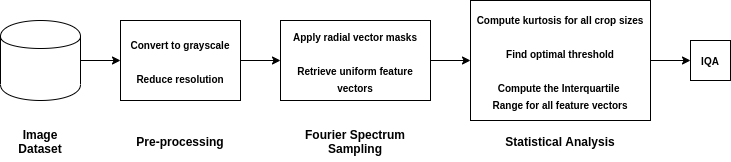
\includegraphics[scale=0.6]{images/nr-iqa_pipeline.png}
  \caption{Pipeline of processing steps of the propose no-reference IQA method.}
  \label{fig:pipeline}
\end{figure}

The DFT was chosen as the basis for the method after tests with the techniques in the literature review, but it was also claimed within the SCG group that it is a simple and robust way to describe image sharpness in terms of a frequency profile. Some tests were done with the discrete wavelet transform, but the response was similar to the DFT. Similarly, after exploring the mathematical properties of the Fourier transform and also the other mathematical functions employed, i.e. the logarithm and the modulus of a complex number, the final feature vector was proven to be a distribution and could be mapped onto a probability space. This discovery brought the idea of statistics to the scope of this work, and by means of visualization techniques such as 2D and 3D plots, it was possible to notice the pattern of blurred and sharp images in the resulting distribution. The need of a statistical property capable of quantifying such pattern and allowing the method to segregate the blurred and sharp images motivated the research for techniques that deal with the shape of a distribution. The simplest tools were kurtosis, the interquartile range and the $z$-score, which were empirically proven to be accurate in the proposed setup.

First, each image undergoes a grayscale conversion with the luminance method \cite{ponti2016image} - a 
linear combination of the three channels of a RGB image, as shown in the matrix equation given by

\begin{equation}
    \label{eqn:luminance}
    I_{luminance} = 0.299R + 0.587G + 0.114B,
\end{equation}

\noindent where $I_{luminance}$ is the matrix that represents the grayscale converted image, $R$, $G$ and $B$ represent the matrices of the red, green and blue channels, respectively. 

The CLAHE algorithm is then applied to deliver a more uniform image to the Fourier Transform. This is necessary as microscopy images are influenced by illumination conditions, the focus adjustment itself and also physical properties of the transmitted or reflected light. Next, the DFT is applied to all images and the resulting spectra are analyzed. The Fourier spectrum of a two-dimensional signal such as an image is a matrix with complex coefficients and zeros on each of its four corners and carries information about frequency bands of the image, characterized as a distribution. Our approach requires a shift between the first and third quadrants, and also the second and the fourth quadrants, to the center of the matrix. The unshifted and shifted Fourier spectrum of an grayscale airplane test image are shown in Figures \ref{fig:fourier_spectrum}.(c) and \ref{fig:fourier_spectrum}.(d), respectively. 

\begin{figure}[ht]
	\centering
	\caption{Original image \textbf{(a)}, luminance grayscale converted image \textbf{(b)}, unshifted Fourier spectrum of the grayscale image \textbf{(c)}, shifted Fourier spectrum of the grayscale image \textbf{(d)} and frequency bands as rings of radius $\{r_{i}: i\in\mathbb{N}^{*}\}$ drawn over the 2D spectrum \textbf{(e)}.}
	\label{fig:fourier_spectrum}
	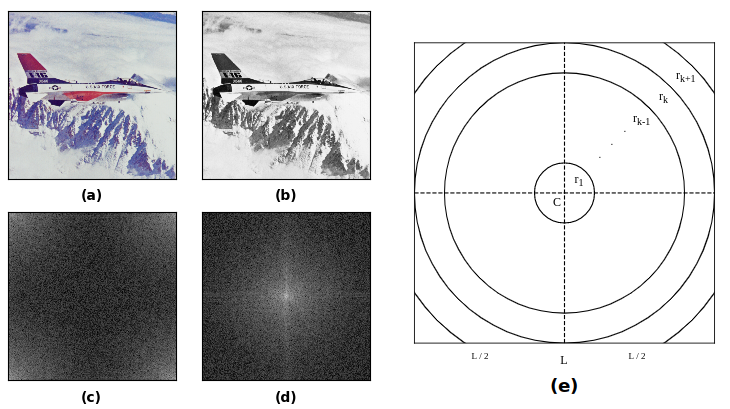
\includegraphics[scale=0.6]{images/fourier_spectrum.png}
	\centering
	\fautor
\end{figure}

The frequency information may be retrieved from the shifted Fourier spectrum by means of concentric circles drawn over it in the form of masks. Theoretically, the number of masks that may be applied to the spectra is infinite, but the discrete nature of images renders a finite number of masks. Let the matrix of DFT coefficients be graphically represented in Figure~\ref{fig:fourier_spectrum}.(e) and be mathematically denoted as a square of side $L = \max{(m,n)}$, $k = L / 2$ be the maximum radius value for circles within the square and $C = (k,k)$ be the center of the infinite set of concentric circles inscribed in the square. Circles with small radii comprise low-frequency information whereas large radii values cover high-frequency coefficients.

Taking into account the pixel resolution of the input images, it makes sense to sample the information, otherwise, the computational complexity and running times of the algorithm for one image alone would be impractical. Moreover, it is also unrealistic to evaluate every area under each concentric circle to retrieve the frequency content of an image; there is also no standard discrete amount of frequency bands to be evaluated. Therefore, we drove our efforts to comprise as much information about each frequency band as possible and explored the fact that the Fourier spectrum of a real function such as an image is even, i.e. symmetric concerning its origin. Instead of the pure complex coefficients, we represent the Fourier spectrum by the magnitude of its coefficients, given by

\begin{equation}
\label{eqn:magnitude_of_DFT}
K(m,n) = 
    \log_{e}{\left(1
    + \sqrt{
        [\operatorname{Re}{(\hat{g}(m,n))}]^{2}
        + [\operatorname{Im}{(\hat{g}(m,n))}]^{2}
      }
    \right)},
\end{equation}

\noindent where $\hat{g}(m,n)$ are the complex Fourier coefficients of an image $g(x,y)$. We propose to sample the spectrum by means of radial lines as masks, i.e. white antialiased lines are drawn over a zero-valued matrix with the same dimensions as the Fourier spectrum of the image, which are then element-wise multiplied by the spectrum. The lines are created from the $(x_{c},y_{c})$ center of the spectrum to points in an approximate radial position, which is calculated by

\begin{equation}
\label{eqn:points_on_radii}
P(x,y) = 
    (
    x_{c} r_{j} \cos{a_{j}}, 
    y_{c} r_{j} \sin{a_{j}}
    )
\end{equation}

\noindent with the set of angles $\{a_{j}\}$ in the radian form, computed as

\begin{align}
\label{eqn:angles}
\left\{
a_{j} : a_{j} = 
\frac{j \pi}{180}
\right\}
&&  j = \{0,10,...,360\}.
\end{align}

Equation
\ref{eqn:points_on_radii} is a
floating-point ordered pair, rounded to the nearest integer value in order to represent a location in the spectrum. The
antialiased lines are drawn with a Gaussian filtering process. After all the lines have been generated, the mask is similar to what is shown in Figure~\ref{fig:radial_masks}:

\begin{figure}[htb]
	\centering
	\caption{Final mask of antialised radial lines to sample the Fourier spectrum.}
	\label{fig:radial_masks}
	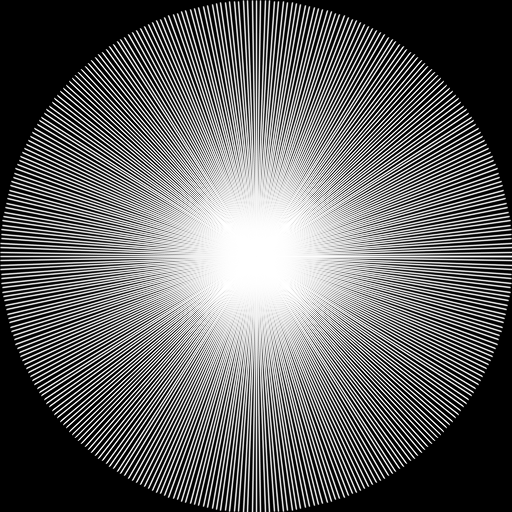
\includegraphics[scale=0.8]{images/radial_masks.png}
	\centering
	\fautor
\end{figure}

The extraction of the region of interest from the spectrum with the mask of radial lines results in arrays of complex coefficients that represent samples of the frequency profile of the image. However, despite the antialiasing, the resulting arrays differ in length since the original data is discrete. The vectors go through an element-wise average, which results in a one-dimensional vector as a descriptor of the frequency spectrum, and before such average, we find the smallest vector size among all of them and discard the remaining information in all of them. For comparison purposes, a square image of side $L$ yields a feature vector of size $1 / 2L$.

Next, the sharpness information of the image is encoded into a low-dimensional and concise representation that may undergo analysis with statistical tools and the mathematical properties of the Fourier spectrum. The feature vectors from each image need to be transformed into a model that is suitable for techniques such as Descriptive Statistics or Bayesian Inference, and therefore must be mapped onto the probability space $\Omega = [0,1]$. Hence, we apply an operator $T : \ell^{2}(\mathbb{Z}^{2}) \rightarrow \ell^{2}(\mathbb{Z}^{2})$, written as

\begin{align}
\label{eqn:probability_operator}
T(x_{i}) = \frac{x_{i}}{\sum_{j=0}^{n-1}x_{j}}
&&  i = \{0,1,...,n-1\},
\end{align}

\noindent where each $x_{i}$ is a value of the descriptor which will be mapped onto a probability. Note that each feature vector after the sampling process is a distribution in the scope of the Distribution Theory, i.e. a continuous linear functional defined on a space of smooth (functions with continuous derivatives up to some desired order over some domain \cite{weisstein2020smooth}) and compact supported (the functions yields zero outside of a closed and bounded set \cite{weisstein2020compact}) functions, with values in the range $[0,\infty)$. Therefore, it makes sense to apply the operator that maps it to a probability. This proposition was proved in \autoref{chapter:definitions-and-proofs}, which summarizes several definitions from Mathematical Analysis, Measure Theory and Distribution Theory required for the proof. The shape of the frequency distribution represented by each descriptor may vary according to the contents of the image, i.e. lines, circles, edges or complex textures, but it possesses a common representation, as shown in \autoref{fig:descriptor} for the 
``1600'' image in the CSIQ database. The black line represents a sharp image (without any degree of Gaussian blur) and the blue line represents the blurriest sample of the ``1600'' subset.

\begin{figure}[htb]
	\centering
	\caption{Common shape of the descriptors right after computation.}
	\label{fig:descriptor}
	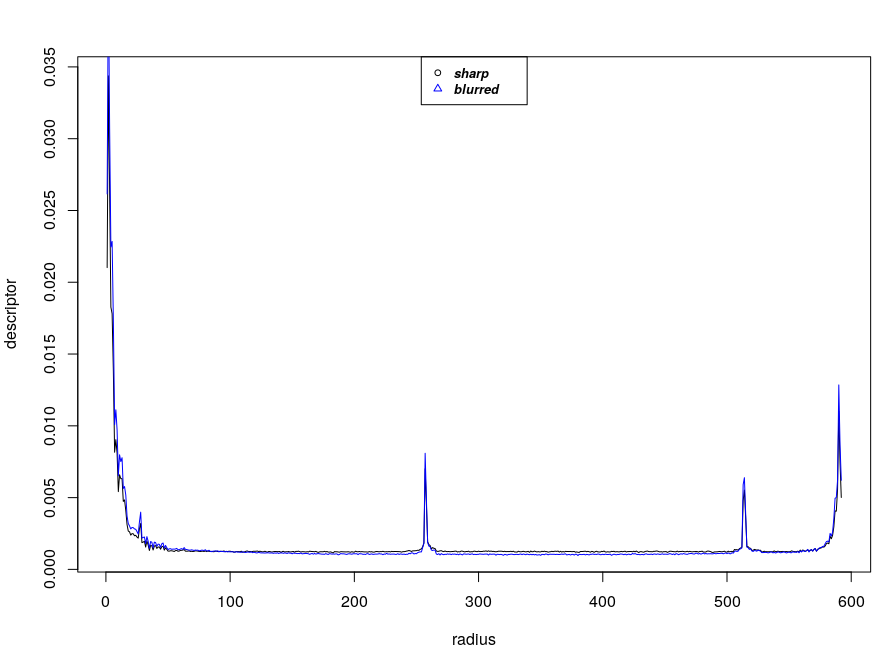
\includegraphics[width=\textwidth, height=12cm, trim = 0cm 0cm 0cm 0.3cm, clip]{images/descriptor.png}
	\centering
	\fautor
\end{figure}

Information embedded in the low-frequency components of each feature vector corresponds to the Dirac delta distribution within the PSF of the microscope and should be discarded since it is equal to all images and does not resemble blur information; the removal should be done with caution so that the remaining information is enough to represent the blur profile of the image and allow the further selection by the image quality metric. An optimal threshold should be calculated for ``cropping'' the data, i.e. only a subset of it will represent the sharpness information. The threshold is chosen to maximize the range of a set of kurtosis values for each feature vector.

Consequently, the data presented by \autoref{fig:descriptor} provides an overview of the distribution of frequencies, but it does not depict distinguishable differences between a sharp and a blurred image. However, by maintaining the range of values, selecting a subset of both sharp and blurred feature vectors (in this case, the dimensions of the original image are $512 \times 512$ and the feature vectors are of length 592) which starts at the position zero and ends at 100, and finally plotting both subsets, it is possible to notice a difference between the graphs. \autoref{fig:low_frequencies} shows that the blue line (the blurred image) contains larger values within the $[0,20]$ interval in the $x$ axis in comparison to the black line (the sharp image), providing less 
``peakedness''  to the distribution - which translates itself as lower kurtosis values.

\begin{figure}[htb]
	\centering
	\caption{Low-frequency profiles of a sharp (black line) and a blurry (blue line) image.}
	\label{fig:low_frequencies}
	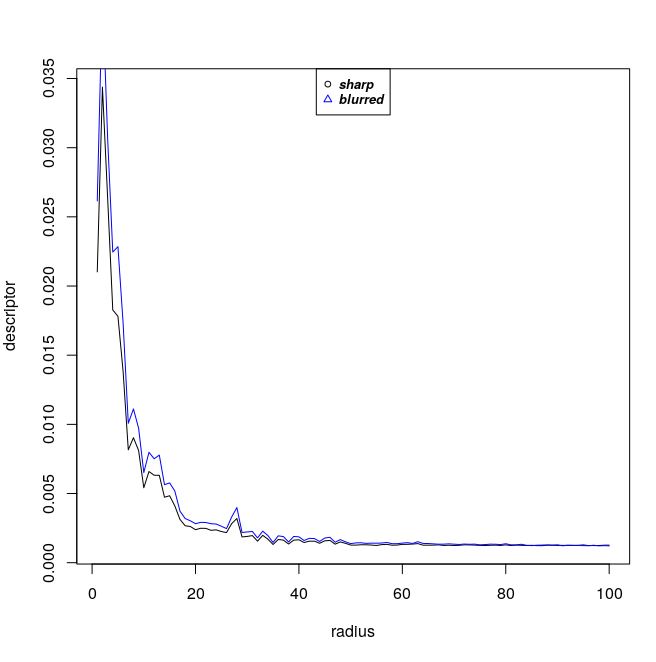
\includegraphics[scale=2.2, trim = 0 0.3cm 0 0.4cm, clip]{images/low_frequencies.png}
	\centering
	\fautor
\end{figure}

The array of kurtosis for every crop size is computed as follows. The crop size initializes as zero and is used to compute the kurtosis of the entire set $\{x_{1},x_{2},...,x_{n}\}$ of all descriptors. The crop size is then incremented by 1, yielding the subset $\{x_{2},x_{3},...,x_{n}\}$. This process is done until the kurtosis for all crop sizes of the feature vectors is computed. Algorithm \ref{alg:kurtosis_array} summarizes the computation of kurtosis for all crop sizes:

\begin{algorithm}[htb]
	\caption{Kurtosis computation}
	\label{alg:kurtosis_array}
	\begin{algorithmic}[1]
	    \State // $X_{c \times n}$: dataset of $n$ descriptors with size $c \in C$, where \\ // $C = \{0,1,...,size(descriptor)\}$ 
	    
	    \\
	    
	    \State // $T(X)$: operator from equation \ref{eqn:probability_operator} to map the \\ // descriptors onto probability distributions
	   
        \\
        
		\State $X \gets T(X)$
		\State $A \gets zeros(c, n)$
		
		\For {\textbf{each} crop size $c$ in $C$}
		    \For{\textbf{each} descriptor $i$ in $\{1,2,...,n\}$}
		
        		\State $A[crop][i] \gets$ \textbf{kurtosis}$\left(X[i].subset(0, crop)\right)$
		
		    \EndFor
		\EndFor
		
		\\
		
		\Return $A$
	\end{algorithmic}
\end{algorithm}

\noindent Next, the optimal threshold computation is done with algorithm~\ref{alg:cut_threshold}. It aims to produce a crop size to maximize the peak to peak value, i.e. the difference between the maximum and minimum values in the dataset. This allows low-frequency information to be discarded from the PSF without loss of the blur.

\begin{algorithm}[ht]
	\caption{Find the optimal dataset variability threshold}
	\label{alg:cut_threshold}
	\begin{algorithmic}[1]
 		\State // $A_{c \times n}$: matrix with kurtosis values for all $n$ descriptors that were computed at every crop \\ // size $c \in C$, where \\ // $C = \{0,1,...,size(descriptor)\}$ 
		
		\\
		
		\State $threshold \gets 0$
		\State $maximum \gets \infty$
		\For {\textbf{each} crop size $c$ in $C$}
		\State $row \gets \{A_{c,1},A_{c,2},...,A_{c,n}\}$ 
		
		\State $a \gets$ \textbf{max}$(row)$
		
		\State $b \gets$ \textbf{min}$(row)$
		
		\\
		
		\If{$a < 0$ or $b < 0$}
		    \State \textbf{continue}
		\EndIf
		
		\\
		
		\State $range \gets a - b$
		
		\\
		
		\If{$range > maximum$}
		    \State $maximum \gets range$
		    \State $threshold \gets c$
		\EndIf
		
		\EndFor
		\\
		\Return $threshold$
% 		\EndFunction
	\end{algorithmic}
\end{algorithm}

The low-frequency is discarded in each feature vector up to the optimal threshold, and a final kurtosis value is computed for all of them. In this work, such final kurtosis value of each feature vector of an image corresponds to the amount of details, i.e. high-frequency content on it: the higher the kurtosis value, the sharper the image is. Finally, an estimate of the subset of images that is eligible for the fusion process is then obtained by the $z$-score transformation by choosing the images that locate at one or more standard deviation units away from the mean.

% IQR measure is computed for all of them. In this work, the IQR value of the feature vector of an image corresponds to the amount of details, i.e. high-frequency content on it: the higher the IQR value, the sharper the image is. Finally, an estimate of the subset of images that is eligible for the fusion process is then obtained by the $z$-score transformation by choosing the images that locate at one or more standard deviation units away from the mean.